\section{Methods}

\begin{frame}
    \frametitle{Fire limitation framework}
    \framesubtitle{Spatial and Temporal controls on fire}

    \begin{tikzpicture}
        \visible<2->{\fill[green, opacity = 0.7] (90:4) -- (210:4) -- (-30:4) -- cycle;}
        \visible<3->{\fill[blue,path fading=west, opacity = 0.7] (90:4) -- (210:4) -- (-30:4) -- cycle;}
        \visible<4->{\fill[red,path fading=south, opacity = 0.7] (90:4) -- (210:4) -- (-30:4) -- cycle;}

        \visible<2>{
            \node (note) at (0,1.5em) {\Huge Fuel Continuity};
            \node (note) at (0,0) { \large fAPAR};
        }

        \visible<3->{
            \node[rotate = 30] at (-2.6,-1.3) {\large Fuel};
            \node[rotate = 30] at (-2.4,-1.6) {fAPAR};
        }

        \visible<3>{
            \node (note) at (0,1.5em) {\Huge Moisture Content};
            \node (note) at (0,0) { \large STASH};
        }

        \visible<4->{
            \node[rotate = -30] at (2.6,-1.3) {\large Moisture};
            \node[rotate = -30] at (2.4,-1.6) {\small STASH};
        }

        \visible<4>{
            \node (note) at (0,1.5em) {\Huge Ignitions};
            \node (note) at (0,0) { \large Lightning};
            \node (note) at (0,-1.25em) { \large Population Density};
            \node (note) at (0,-2.5em) { \large Pasture};
        }

        \visible<5->{
            \node[anchor = east, rotate = 90] at (-1em,3.3) {\large Ignitions};
            \node[anchor = east, rotate = 90] at (0,3.3) {\small Lightning};
            \node[anchor = east, rotate = 90] at (1em,3.3) {\small PopDens, Pasture};
        }

        \visible<5>{
            \node (note) at (0,0) {\Huge Burnt Area};
        }

    \end{tikzpicture}


    \begin{textblock*}{5cm}(6.67cm,2cm)
        \visible<6->{
            \begin{tikzpicture}[scale=0.67]
                \fill[green] (90:4) -- (210:4) -- (-30:4) -- cycle;
                \fill[blue,path fading=west] (90:4) -- (210:4) -- (-30:4) -- cycle;
                \fill[red,path fading=south] (90:4) -- (210:4) -- (-30:4) -- cycle;
                \fill[black, opacity = 0.5] (90:4) -- (210:4) -- (-30:4) -- cycle;
            \end{tikzpicture}
        }
    \end{textblock*}

    \begin{textblock*}{5cm}(10.1cm,2cm)
        \visible<7->{
            \begin{tikzpicture}[scale=0.33]
                \fill[green] (90:4) -- (210:4) -- (-30:4) -- cycle;
                \fill[blue,path fading=west] (90:4) -- (210:4) -- (-30:4) -- cycle;
                \fill[red,path fading=south] (90:4) -- (210:4) -- (-30:4) -- cycle;
                \fill[black, opacity = 0.8] (90:4) -- (210:4) -- (-30:4) -- cycle;
            \end{tikzpicture}
        }
    \end{textblock*}

    \begin{textblock*}{4.5cm}(4.6cm,2.6cm)
        \visible<6->{
            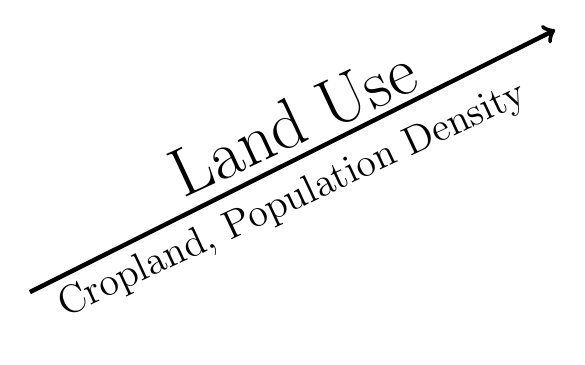
\begin{tikzpicture}
                \node[rotate = 25 ] (note) at (3.335, 2.165) {\Huge Land Use};
                    \node[rotate = 25 ] (note) at (3.335, 1.165) {\Large Cropland, Population Density};
                \draw[ultra thick, ->] (0, 0) -- (6.67, 3.33);
            \end{tikzpicture}
        }
    \end{textblock*}

    %Stuff to include:
    %   Monthly -> Inter annual and seasonal controls
\end{frame}
